\section{Appendix}
\label{sec:appendix}

\subsection{Detailed Analysis on Universal Target Generation}
\label{app:detailed-universal-target}
The goal of a universal target is to be sufficiently close in latent image space for each frame to optimize towards. In Figure~\ref{fig:target-selection-algorithm-results}, we plot the latent $L_2$ norm between each frame in a scene to a universal target generated by three different methods. We find that simple pixel averaging generates universal target images that are consistently closer to all frames in a scene, and thus adopt it for our evaluation section.

\begin{figure}[h]
    \centering
    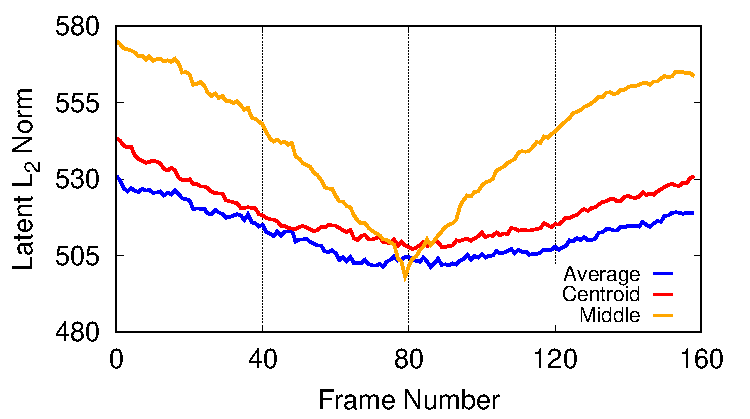
\includegraphics[width=0.8\columnwidth]{plots/eval/scene-targets-eps-converted-to.pdf}
    \vspace{-0.15in}
    \caption{Generating a single target image by pixel averaging all images in a scene leads to the least amount of fluctuation and distance in latent $L_2$ norm between each frame to the target image.}
    \label{fig:target-selection-algorithm-results}
\end{figure}

\begin{figure*}[t]
    \centering
    \begin{minipage}[t]{0.49\textwidth}
    \centering
    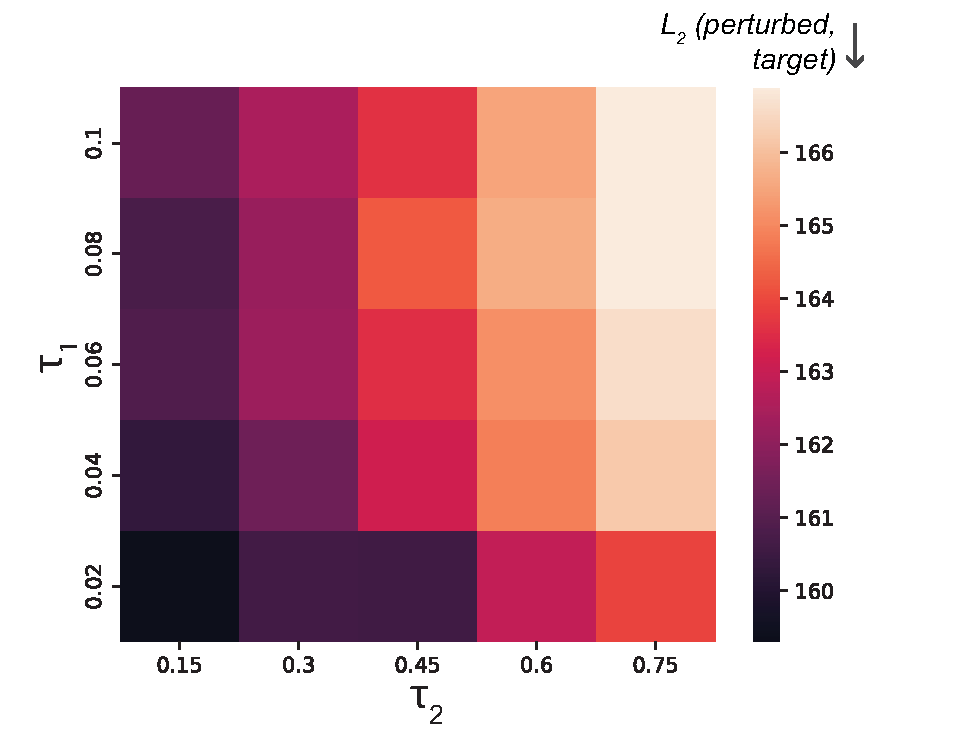
\includegraphics[width=0.9\columnwidth]{plots/heatmaps/flurdeh-adv-performance-eps-converted-to.pdf}
    \vspace{-0.1in}
    \caption{Gridsearch of \system's two threshold parameters $\tau_1, \tau_2$ with respect to the latent $L_2$ norm between perturbed frames and the target it is optimized towards. A lower latent $L_2$ norm equates to better optimized perturbation and stronger robust protection. Decreasing both values leads to higher number of full optimizations, and stronger robustness.}
    \label{fig:grid-search-robustness}
    \end{minipage}
    \hfill
    \centering
    \begin{minipage}[t]{0.49\textwidth}
    \centering
    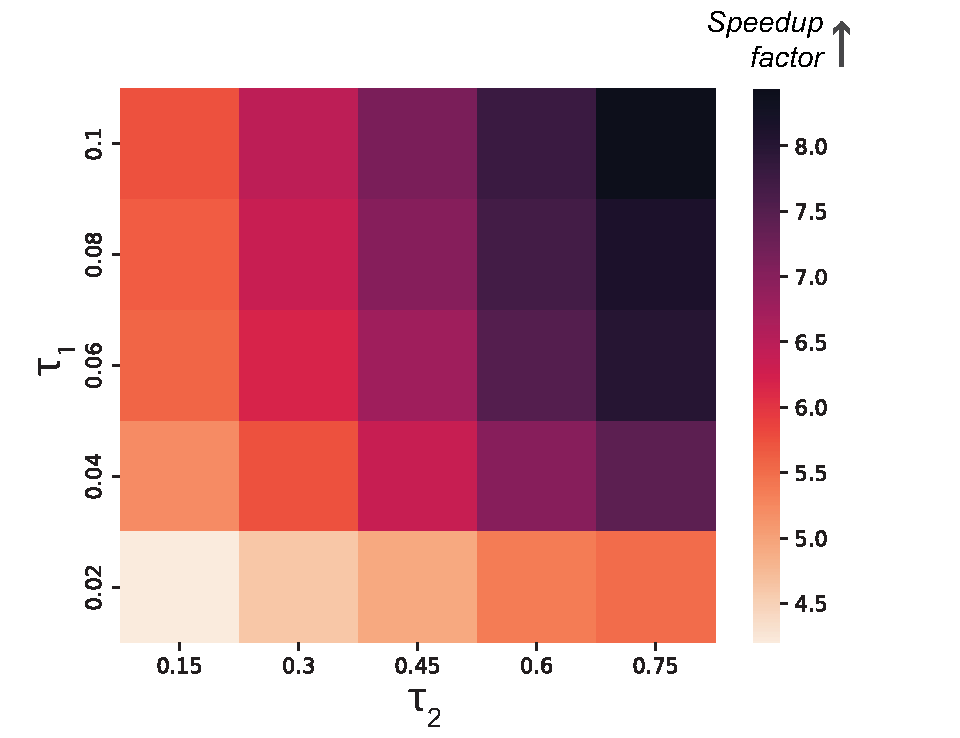
\includegraphics[width=0.9\columnwidth]{plots/heatmaps/flurdeh-adv-speedup-eps-converted-to.pdf}
    \vspace{-0.1in}
    \caption{Gridsearch of \system's two threshold parameters $\tau_1, \tau_2$ with respect to the computation speedup. Increasing both values leads to less number of full optimizations, and more significant speedup.}
    \label{fig:grid-search-robustness}
    \label{fig:grid-search-efficiency}
    \end{minipage}
      \hfill
\end{figure*}

\begin{figure*}[t]
  \centering
  \begin{minipage}[t]{0.32\textwidth}
  \centering
  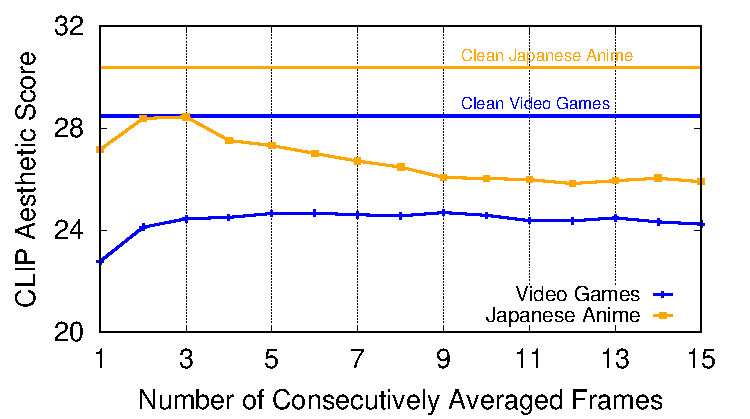
\includegraphics[width=0.9\columnwidth]{plots/avg-tests/avg-aesthetic-eps-converted-to.pdf}
  \vspace{-0.1in}
  \caption{Average image quality (CLIP Aesthetic score) increases initially as the number of consecutively frames used for averaging attack increases, but decreases after too many frames are averaged for both Video Game and Japanese Anime videos.}
  \label{fig:aesthetic-caf}
  \end{minipage}
  \hfill
  \centering
  \begin{minipage}[t]{0.32\textwidth}
  \centering
  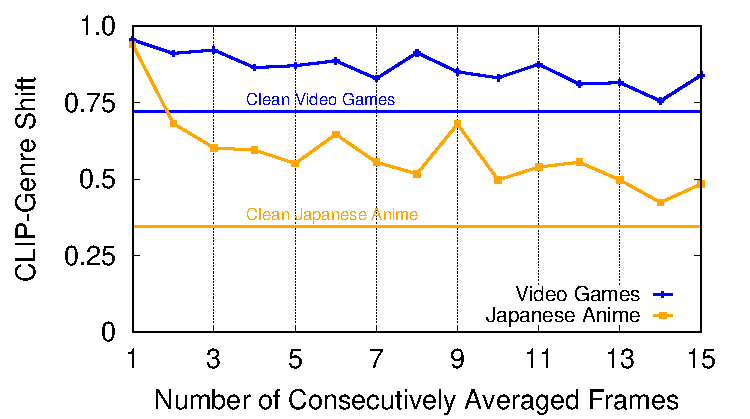
\includegraphics[width=0.9\columnwidth]{plots/avg-tests/avg-clip-shift-eps-converted-to.pdf}
  \vspace{-0.1in}
  \caption{Average robustness (CLIP-Genre Shift) decreases as the number of consecutively frames used for averaging attack increases and stagnates as more frames are used for both Video Game and Japanese Anime videos.}
  \label{fig:clip-shift-caf}
  \end{minipage}
    \hfill
    \centering
  \begin{minipage}[t]{0.32\textwidth}
  \centering
  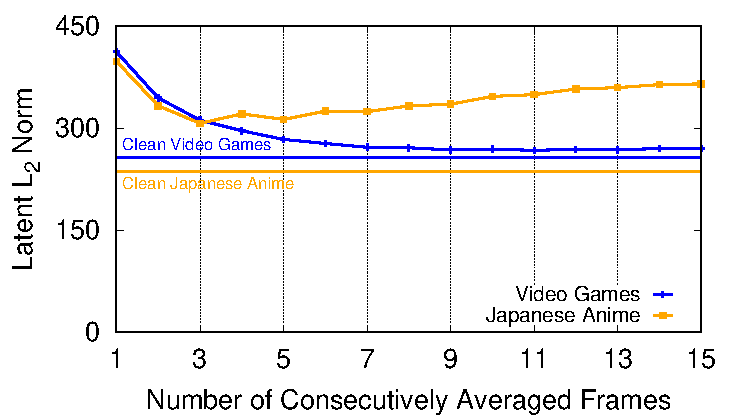
\includegraphics[width=0.9\columnwidth]{plots/avg-tests/avg-l2-eps-converted-to.pdf}
  \vspace{-0.1in}
  \caption{Average latent $L_2$ norm between perturbed frames and clean frames initially decreases as the number of consecutive frames used for averaging attack increases. The benefit stagnates for Video Game videos, but loses effectiveness for Japanese Anime.}
  \label{fig:l2norm-caf}
  \end{minipage}
    \hfill
\end{figure*}

\subsection{Detailed Perturbation Removal Attacks}
\label{app:detailed-perturbation-removal}

\para{FILM}
Frame Interpolation for Large Motion (FILM)~\cite{reda2022film} is a neural network designed to generate slow motion videos from two ``near duplicate'' images. FILM adapts a multi-scale feature extractor to estimate scale-agnostic motion, allowing the synthesis of high quality intermediate frames. While there are many SOTA film interpolation softwares available ~\cite{niklaus2020softmax, bao2019depth, huang2022real}, these focus largely on estimating motion and optical flow. In contrast, FILM prioritizes generating sharp, high quality videos by using Gram matrix loss ~\cite{gatys2016image} to fill in the gap between two or more images. We implement their code to generate a single interpolated image between two images separated five frames apart. FILM is designed to handle both large and small motion, thus we find that the distance between frames does not impact the success of this removal attack.

\para{Simple Linear Interpolation}
We apply a simple linear interpolation function to generate a new image by smoothly blending the pixel values of two input images. We chose an interpolation factor $\alpha = 0.5$ to give equal weight to both images. Similar to our existing perturbation removal attacks, we perform simple linear interpolation between two images 5 frames apart. 

\subsection{Number of Images to use in Average Attack}
\label{app:num-images-average}
Figures \ref{fig:aesthetic-caf}-\ref{fig:l2norm-caf} plot the robustness and quality of protected images as a function of the number of consecutive frames used by our selective pixel averaging attack. Image quality begins to degrade when more than 3-5 consecutive frames are used for selective pixel averaging, with diminishing returns on recovering the correct artist style. Thus, we fix the number of averaged frames to 5 throughout our evaluation.

\subsection{User Study Detailed Description}
\label{app:detailed-user-study}
\para{Ethics}
We conduct two IRB-approved user studies. The first study, released on Twitter, involved 305 volunteers from the art community who rated the effectiveness of \system~ compared to naive perturbations in protecting videos against style mimicry attempts. We only presented style-mimicked images from the Video Game and Japanese Anime datasets, chosen due to their relevance to current threats faced by video creators as discussed in \S\ref{sec:intro}. These datasets align with art content that existing image protection systems (Glaze, Mist, AntiDB \cite{shan2023glaze,mist,antidb}) are designed to safeguard.

The second study, conducted on Prolific, involved 220 participants who were presented with style-mimicked images from videos across all 5 datasets. They were compensated at \$12 per hour and filtered for English-Speaking participants in the US, over the age of 18 and with over 95\% approval rating on Prolific.

All videos from these datasets are publicly available on YouTube, and we strictly use them for research purposes.

\subsection{Choosing System Parameters}
\label{app:system-parameters}
This is a detailed explanation on the selection of two threshold parameters introduced in \S\ref{subsec:system-parameters}. We perform a grid search on 25 combinations of \system's two threshold parameters using Glaze as the image perturbation algorithm, and measure the average robustness and speedup that each achieves. In Figures \ref{fig:grid-search-robustness} and \ref{fig:grid-search-efficiency}, we find that there is an intuitive reverse tradeoff between robustness and computation efficiency. Decreasing both parameters leads to more computations of perturbations from scratch, which benefits robustness but incurs slower speedup. Assuming that video content creators must balance these two objectives, we choose the middle parameters, $\tau_1 = 0.06$ and $\tau_2 = 0.45$, to use in our evaluation.


\subsection{Averaging Images Degrades Mimicry Quality}
Here, we investigate the impact that our averaging attack on style mimicry models trained on clean images. We take clean unperturbed frames of four videos from the Japanese Anime dataset and perform our averaging attack on the 5 frames surrounding each high quality frame used in style mimicry. Our results show that the average attack on clean images causes CLIP-Genre Shift to increase from 0.15 to 0.19. This suggest that our average attacks slightly weakens style mimicry, which is supported by natural blurring caused by movement and inter-frame changes. Additionally, this result helps explain why averaging attack on \system~ has higher CLIP-Genre Shift scores when compared to naive perturbation methods. \system~ successfully protects against averaging attack, but style mimicry is also compounded by the natural degradation of image quality when averaging attack is used.

\subsection{Increasing $\tau_2$ Degrades Robustness}
\label{app:eps-robustness}
In \S\ref{subsec:protection-usability}, we show that speedup from \system~ can be significantly improved by increasing our second threshold parameter $\tau_2$. While our grid search signals that increasing either threshold parameter leads to lower robustness via. latent $L_2$ norm, we also show that increasing $\tau_2$ leads to worse robustness on end to end style mimicry models. On the same four Japanese Anime videos used to evaluate computation efficiency in \S\ref{subsec:protection-usability}, the default $\tau_2 = 0.45$ results in average CLIP-Genre Shift score of 0.95, while increasing $\tau_2 = 0.8$ drops CLIP-Genre Shift score to 0.90. 


